\documentclass[11pt,a4paper]{article}
\usepackage[utf8]{inputenc}
\usepackage{amsmath}
\usepackage[czech]{babel}
\usepackage{amsfonts}
\usepackage{amssymb}
\usepackage{graphicx}
\usepackage{subcaption}
\usepackage{a4wide}
\usepackage{siunitx}
\usepackage{booktabs}
\usepackage{float}
\usepackage{empheq}
\usepackage[most]{tcolorbox}
\newtcbox{\mymath}[1][]{%
	nobeforeafter, math upper, tcbox raise base,
	enhanced, colframe=blue!30!black,
	colback=blue!30, boxrule=1pt,
	#1}
\usepackage[figurename=Obr., tablename=Tab.]{caption}
\sisetup{output-decimal-marker = {,}}
\usepackage[version=4]{mhchem}
\usepackage[colorlinks=true,urlcolor=black,citecolor=blue]{hyperref}
%\usepackage{cleveref}
\author{Michal Šesták}
\title{Čip v sudu s radonovou atmosférou}
\begin{document}
\maketitle	
\tableofcontents
\section{Úvod}
Účelem tohoto experimentu je zkoumání vlivu kosmického záření na chybovost integrovaného obvodu. Kosmické záření je simulováno radonovou atmosférou v plechovém uzemněném sudu válcové geometrie, v jehož středu je čip umístěn. Radonová atmosféra je vytvořena injekcí definované koncentrace radonu do sudu v daný počáteční čas. Kolem čipu jsou umístěny TLD detektory, kterými měříme dávku absorbovanou v čipu. Dále se měří počet chyb zaznamenaných v různých segmentech čipu, např v ADC nebo v paměti. Snahou je zjistit, zdali existuje nějaká závislost počtu chyb v čipu na velikosti absorbované dávky.

Problémem je, že zatímco $\beta$ a $\gamma$ záření je TLD detektory měřeno spolehlivě, u $\alpha$ tomu tak není. Proto se přistoupilo k pokusu o výpočet dávky z jednotlivých složek záření ($\alpha, \beta, \gamma$) pomocí teoretických poznatků. 

Ještě předtím však bylo potřeba ověřit, že radon difunduje do zkoumaného čipu přes vrstvičku materiálu, která ho obklopuje, dostatečně rychle vzhledem k jeho radioaktivní přeměně. Pokud by difundoval mnohem pomaleji než se přeměňuje, pak by dávka (hlavně její část pocházející od alf) byla nižší než v případě, kdy bychom uvažovali stejnou koncentraci radonu v čipu jako v okolním prostředí sudu. Proto byl výpočet dávky rozdělen do dvou úloh.
\section{Úlohy}
\begin{enumerate}
	\item Ověření, zdali radon difunduje k čipu přes vrstvičku materiálu pouzdra dostatečně rychle vzhledem k radioaktivní přeměně radonu v sudu.
	\item Výpočet dávky absorbované v čipu. Určují se jednotlivě příspěvky od záření $\alpha, \beta, \gamma$.
\end{enumerate}
\clearpage
\section{Difúze radonu do čipu skrze pouzdro}
\subsection{Popis difúzního šíření}
Průběh šíření radonu difúzí v čase v daném materiálu popsaném difúzním součinitelem $D$ se řídí druhým Fickovým zákonem
\begin{equation}
\frac{\partial c}{\partial t}=D\cdot \text{div}(c)-\lambda c\,,\label{eq:fickuvLawObecne}
\end{equation}
kde $c=c(t;x,z,y)$ je koncentrace radonu v bodě $(x,y,z)$ v čase $t$, $\lambda$ je přeměnová konstanta radonu; $[c]=\si{Bq/m^3}$; $[D]=\si{m^2s^{-1}}$. 

\subsection{Součinitel difúze a rozměry čipu a pouzdra}\label{rozmery}
Vzhledem k tomu, že známe pouze prvkové složení pouzdra a nevíme, z jakého materiálu je vyrobeno, tak byl uvažován difúzní součinitel o hodnotě
\begin{equation}
D=\SI[parse-numbers = false]{3\cdot 10^{-7}}{m^2s^{-1}}\,,
\end{equation}
což by měla být hodnota obvyklá pro pevné látky (zdroj?\footnote{zkusit najít a doplnit}). Čip je rozměrově kvádr o šířce a délce cca 7 mm a tloušťce 0,15 mm. Pouzdro ho obepíná, na bočních stranách čipu je 6,5 až 7 mm materiálu pouzdra, na horní a dolní ploše čipu je ho 0,69 mm. 

\subsection{Numerické řešení difúzní rovnice}\label{pol:aproximace}
Řešení rovnice \eqref{eq:fickuvLawObecne} v kartézských souřadnicích při daných rozměrech pouzdra by bylo zbytečně náročné, a proto se přistoupilo k aproximaci čipu koulí o poloměru $R_1$ a pouzdra kulovou slupkou o poloměru $R_2$ a tloušťce $d$. Pak lze rovnici \eqref{eq:fickuvLawObecne} převést do sférických souřadnic $(r, \varphi, \phi)$ s počátkem ve středu aproximujících útvarů:
\begin{equation}
\frac{\partial c}{\partial t}=D\left(\frac{\partial^2c}{\partial r^2}+\frac{2}{r}\frac{\partial c}{\partial r}\right)-\lambda c\,,\label{eq:fick}
\end{equation}
kde navíc díky homogennosti koncentrace radonu v okolí pouzdra uvažujeme izotropní šíření, tj. nezávislé na souřadnicích $\varphi$ a $\phi$, a proto $c=c(t,r)$. V prvním přiblížení byly aproximující parametry položeny hodnotám
\begin{align}
	R_1&=\SI{5}{cm}\,,\\
	R_2&=\SI{10}{cm}\,,\\
	d=R_2-R_1&=\SI{5}{cm}\,,
\end{align}
v případě potřeby by byly zmenšeny. Rovnice \eqref{eq:fick} byla řešena jen uvnitř pouzdra. 
\subsubsection{Počáteční a okrajové podmínky}
Byly řešeny dva případy:
\begin{enumerate}
	\item \textbf{Injektáž radonu:} v okolí čipu je konstantní koncentrace radonu $c_0$ a uvnitř čipu a pouzdra je v počátečním čase nulová koncentrace, tj.:
	\begin{itemize}
		\item počáteční podmínka je $c(0,r)=c_u(0)=0$ pro $r\in(R_1, R_2)$, kde $c_u(t)$ je koncentrace radonu v kouli aproximující čip v blízkosti pouzdra,
		\item okrajová podmínka na rozhraní pouzdra a okolního prostředí (dále jen vnější okrajová podmínka) je $c(t,R_2)=c_0$ pro $t\in[0,T]$, kde $T$ čas, do kterého chceme rovnici řešit,
		\item okrajová podmínka na rozhraní pouzdra a čipu (dále jen vnitřní okrajová podmínka) bude uvedena později.
	\end{itemize}
	 
	\item \textbf{Vypumpování radonu:} v okolí čipu je nulová koncentrace radonu a uvnitř čipu a pouzdra je koncentrace tentokrát v počátečním čase $c_0$, tedy:
	\begin{itemize}
		\item počáteční podmínka je $c(0,r)=c_u(0)=c_0$ pro $r\in[R_1, R_2]$,
		\item vnější okrajová podmínka je $c(t,R_2)=0$ pro $t\in[0,T]$,
		\item vnitřní okrajová podmínka bude uvedena později.
	\end{itemize} 
\end{enumerate}
První případ představuje injektáž radonu do sudu s čipem, druhý pak vypumpování radonu ven ze sudu. Vnitřní okrajová podmínka vypadá následovně:
\begin{equation}
	D\frac{\partial c(t,R_1)}{\partial r}=h\cdot(c(t,R_1)-c_u(t))\,,\label{eq:vnitrniOkrPodm}
\end{equation}
kde $h$ je tzv. přestupní koeficient vyjadřující schopnost přestupu radonu z pouzdra do čipu (nebo naopak), $[h]=\si{m\cdot s^{-1}}$. Jeho určení je velmi problematické a v podstatě nebyla provedena žádná systematická měření jeho hodnot pro rozhraní různých materiálů. Autoři článku~\cite{jiranek1} odhadují jeho hodnotu pro nezměřená rozhraní na
\begin{equation}
	h=\SI{0,1}{m\cdot s^{-1}}\,,
\end{equation}
tato hodnota byla uvažována i v našich výpočtech.

Koncentrace uvnitř čipu $c_u(t+\Delta t)$ se určí ze známé koncentrace v předchozím bodě časové sítě $c_u(t)$ pomocí vztahů
\begin{align}
	E(t)&=h\cdot(c(t,R_1)-c_u(t))\,,\label{eq:exhalace}\\
	c_u(t+\Delta t)&=c_u(t)\cdot \mathrm{e}^{-\lambda\Delta t}+\frac{E(t)\cdot A}{V\cdot \lambda}\cdot \left(1-\mathrm{e}^{-\lambda\Delta t}\right)\,,\nonumber\\
	&=c_u(t)\cdot \mathrm{e}^{-\lambda\Delta t}+\frac{3\cdot E(t)}{R_1\cdot \lambda}\cdot \left(1-\mathrm{e}^{-\lambda\Delta t}\right)\,,\label{eq:vnitrek}
\end{align}
kde $E(t)$ exhalační rychlost z pouzdra do čipu (či naopak) v čase $t$, $[E]=\si{Bq\cdot m^{-2}s^{-1}}$, dále $\Delta t$ je časový krok, $\lambda$ je přeměnová konstanta radonu, $A=4\pi R_1^2$ je vnější plocha koule reprezentující čip a $V=\frac{4}{3}\pi R_1^3$ je objem této koule. Vztahy \eqref{eq:vnitrniOkrPodm}, \eqref{eq:exhalace} a \eqref{eq:vnitrek} byly převzaty z \cite{jiranek1}.

Vnější okrajová podmínka představuje Dirichletovu okrajovou podmínku, vnitřní pak Neumannovu okrajovou podmínku.
\subsubsection{Použitá metoda}
Pro určení prostorového a časového vývoje koncentrace v pouzdře $c(t,r)$ pro $t\in[0, T], r\in[R_1, R_2)$ a časového vývoje koncentrace uvnitř čipu v blízkosti pouzdra $c_u(t)$ pro $t\in[0,T]$ z rovnic \eqref{eq:fick}, \eqref{eq:vnitrniOkrPodm} a \eqref{eq:vnitrek} byla použita Crank-Nicolsonova metoda \cite{numerical_methods, wiki}. 

Z takto určeného vývoje je možné stanovit dobu $T_1$, resp. $T_2$ (pro první a druhý případ), po níž bude radon difundovat přes pouzdro do čipu, dokud nebude v čipu s určitou tolerancí $\varepsilon$ stejná koncentrace radonu jako ve vnějším prostředí. Při výpočtu byla použita tolerance
\begin{equation}
	\varepsilon=0,01\,.
\end{equation}
\subsection{Výsledek}
\begin{figure}[t!]
	\centering
	\begin{subfigure}{.7\textwidth}
		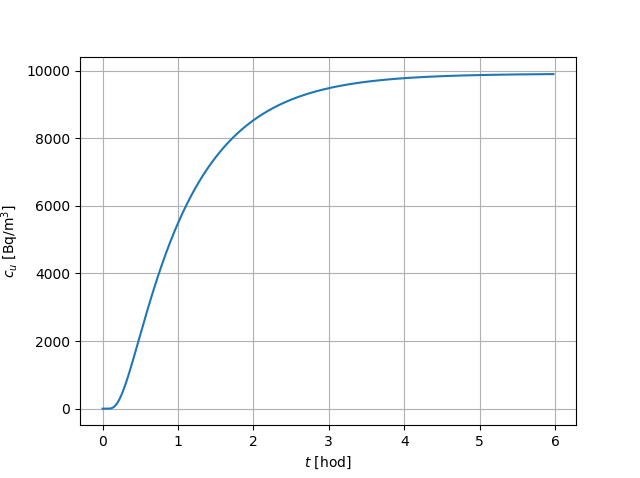
\includegraphics[width=\linewidth]{narust}
		\caption{}
		\label{fig:narust}
	\end{subfigure}
	\begin{subfigure}{.7\textwidth}
		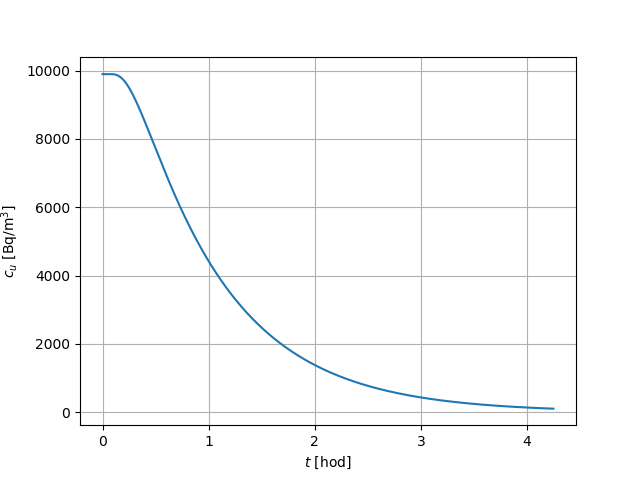
\includegraphics[width=\linewidth]{pokles}
		\caption{}
		\label{fig:pokles}
	\end{subfigure}
\caption{V (a) je vidět časový vývoj koncentrace radonu v čipu v bezprostřední blízkosti pouzdra v prvním uvažovaném případě (injektáž radonu). V (b) je vidět vývoj $c_u$ pro druhý případ (vypumpování radonu ze sudu ven). V obou případech uvažujeme $c_0=\SI{10}{kBq/m^3}$.}
\label{fig:vyvoj_uvnitr}
\end{figure}
Časový vývoj $c_u$ je pro oba dva případy k nahlédnutí v obr.~\ref{fig:vyvoj_uvnitr}. $T_1$ a $T_2$ vychází pro všechna testovaná $c_0$ stejně:
\begin{align}
	T_1&=\SI{5,98}{hod}\,,\\
	T_2&=\SI{4,25}{hod}\,,\\
	T_1+T_2&=\SI{10,23}{hod}\,,
\end{align}
doba $T_1+T_2$ představuje celkovou dobu trvání obou případů. Byly testovány následující hodnoty $c_0$: $\SI{1}{kBq/m^3}, \SI{10}{kBq/m^3}, \SI{100}{kBq/m^3}, \SI{1}{MBq/m^3}$
\subsection{Diskuze}
Doby $T_1$, $T_2$ a $T_1+T_2$ jsou v porovnání s $T_{1/2}(\ce{^{222}Rn})=\SI{3,82}{dne}$ krátké. Vzhledem k tomu že výpočet proběhl pro mnohem větší rozměry pouzdra než jaké ve skutečnosti jsou, tak můžeme říct, že v čipu je stejná koncentrace radonu jako v sudu po většinu času experimentu. Toto tvrzení ovšem platí pouze za předpokladu, že uvažovaný součinitel difúze skrze pouzdro $D$ není hodně nadhodnocený.
\subsection{Závěr}
Bylo ověřeno, že radon difunduje skrze pouzdro do čipu dostatečně rychle vzhledem k radioaktivní přeměně radonu.
\begin{thebibliography}{Mm99}
	\bibitem{jiranek1} Jiránek M., Fronka A.: New technique for the determination of radon diffusion coefficient in radon-proof membranes. Radiat Prot Dosimetry. 2008;130(1):22-5. doi: 10.1093/rpd/ncn121.
	\bibitem{numerical_methods} Hellevik, L. R.: Numerical Methods for Engineers. Department of Structural Engineering, NTNU. 2018. Citováno 10. 5. 2019. Dostupné z \url{http://folk.ntnu.no/leifh/teaching/tkt4140/._main068.html#ch5:sec6} a \url{http://folk.ntnu.no/leifh/teaching/tkt4140/._main069.html#ex:52}
	\bibitem{wiki} Wikipedia, The Free Encyclopedia: Crank–Nicolson method. Citováno 10. 5. 2019. Dostupné z \url{https://en.wikipedia.org/wiki/Crank%E2%80%93Nicolson_method}
	\end{thebibliography}
\clearpage
\section{Výpočet dávky absorbované v čipu}
I v této úloze aproximuje čip a pouzdro koulemi se středy ve stejném bodě, zde však s poloměry $R_1$, resp. $R_2$:
\begin{align}
	R_1&=\SI{3,0}{mm}\,,\\
	R_2&=\SI{3,1}{mm}\,,
\end{align}
které odpovídající více reálným rozměrům čipu a pouzdra (lze dohledat v oddíle \ref{rozmery}). Objem a hmotnost čipu jsou označeny jako $V_{cip}$ a $m_{cip}$:
\begin{align}
	V_{cip}&=\SI{0,0073}{cm^3}\,,\\
	m_{cip}&=\SI{1.7e-05}{kg}\,.
\end{align}
Při výpočtu $m_{cip}$ bylo uvažováno, že celý čip je z křemíku. 

Sud je válec o poloměru a výšce
\begin{align}
R_{sud}&=\SI{27}{cm}\,,\\
h_{sud}&=\SI{83}{cm}\,
\end{align}
a jeho objem je
\begin{align}
	V_{sud}=\SI{0,19}{m^3}\,.
\end{align}

Uvažujeme několik hodnot faktoru nerovnováhy: $F=\num{0,01};\ \num{0,1};\ \num{0,4}$. Objemová aktivita radonu je označena $a$. Do sudu je na začátku experimentu jednorázově injektována počáteční koncentrace radonu $a_0$, průběh $a$ v sudu se pak řídí zákonem exponenciální přeměny.
\subsection{Příspěvek od $\alpha$}
V následujících dvou podkapitolách budou určeny energetické příspěvky od $\alpha$ částic vzniklých mimo a uvnitř čipu, resp. pouzdra, při dané aktivitě $a_0$ za jednotkový časový interval (tj. \SI{1}{s}). V následující podkapitole proběhne časová integrace těchto příspěvků přes zadanou dobu expozice a následné podělení hmotností pro určení dávky od $\alpha$ částic.
\subsubsection{Energetický příspěvek od $\alpha$, které vznikly mimo čip a pouzdro}\label{navesti:algoritmus_nabiteCastice}
Částice $\alpha$ o dané počáteční energii $T_0$ má v daném prostředí známý maximální dosah $R_{max}$~\cite{astar}. Proto lze okolo čipu uvažovat kouli o poloměru 
$$R_3=R_{max}+R_2\,,$$
v jejímž objemu vzniklé alfa částice mohou dolétnout k pouzdru. Alfa částice emitované mimo tuto kouli budou zastaveny dříve než doletí k pouzdru čipu. Ztrátu energie částice alfa, která vznikla ve vzdálenosti $r\in[R_2, R_3]$ od pouzdra, po projití vrstvy vzduchu o tloušťce $r$ je možné zjistit z tabelovaných hodnot brzdných schopností \cite{astar} a pomocí následujícího jednoduchého algoritmu:
\begin{enumerate}
	\item \emph{Inicializace}:
	\begin{align*}
	x&=0\,,\\
	  dE&=0\,,\\
	   dx&=0,1\,.
	   \end{align*}
	  $x$ je doposud ušlá dráha alfa částice; $dE$ je ztráta energie, která je vypočítávána v každé iteraci; $dx$ je krok, my jej bereme roven jednomu milimetru.
	\item \emph{Iterace}:
	\begin{align}
		x = x+dx\,,
	\end{align}
	kontrola $x<r$,
	\begin{align*}
	dE &= \frac{dE}{dx}(T_i)\cdot dx\,,\\    
	T_{i+1} &= T_i - dE\,,
	\end{align*}  
	kontrola $dE>0$ a $T_{i+1}>0$. 

$\frac{dE}{dx}(T_i)$ je brzdná schopnost alfa částice o energii $T_i$ ve vzduchu. Spojitá závislost $\frac{dE}{dx}$ na $T$ byla získána interpolováním tabelovaných hodnot z~\cite{astar} kubickým splinem.
\item \emph{Ukončení cyklu}:\\
pokud byla porušena jakákoliv kontrola v předchozím bodě, pak je cyklus ukončen a momentální $T$ je energie, která alfa částici zbyla při příchodu k pouzdru.
\end{enumerate}

Předchozí algoritmus je vlastně funkcí vzdálenosti vzniku alfa částice od pouzdra, tj. $r$, označme tuto funkci $f_0(r)$. Po přenásobením korekcí na prostorový úhel
\begin{equation*}
k_1=\frac{1}{2}\cdot\left(1-\frac{r}{\sqrt{r^2+R_1^2}}\right)\,,
\end{equation*}
a faktorem zohledňujícím skutečnost, že nás zajímají alfy z celé slupky s vnitřním poloměrem $r$ a vnějším poloměrem $r+\mathrm{dr}$
\begin{equation*}
	k_2=4\pi r^2\,,
\end{equation*}
získáváme funkci $f(r)$, kterou lze zintegrovat od $R_2$ do $R_3$, tj.
\begin{equation}
	I=\int_{R_2}^{R_3}f(r)=\int_{R_2}^{R_3}k_1(r)\cdot k_2(r)\cdot f_0(r)\mathrm{dr}\,. 
\end{equation}
Tato veličina představuje střední hodnotu zbylé energie alfa částice s danou počáteční energií $T_0$ po dojití k pouzdru, která je přenásobená objemem kulové slupky s poloměry $R_2$ a $R_3$ a její rozměr je tedy 
\begin{equation}
	[I]=\si{MeV\cdot cm^3}\,.
\end{equation}

Po vydělení $I$ integrovaným objemem  $V=\frac{4}{3}\pi(R_3^3-R_2^3)$ získáváme střední energii alfa částice u vstupu do pouzdra:
\begin{equation}
	\bar{E}=\frac{I}{V}\,.
\end{equation}
Vypočítané hodnoty $I$, $\bar{E}$ a počáteční kinetické energie $T_0$ alfa částic emitovaných radonem a jeho krátkodobě žijících dceřinných produktů jsou v tabulce~\ref{tab:alfa_energie}.
\begin{table}[ht]
	\centering
	\caption{Počáteční energie, $I$ a $	\bar{E}_{pouzdro}$ alfa částic emitovaných radonem a jeho krátkodobě žijícími dceřinnými produkty (RN=radionuklid).}
	\label{tab:alfa_energie}
	%3.1635352 , 4.10481408, 8.36293245
	%0.00836222, 0.00737454, 0.00493332
	\begin{tabular}{lrrr}
		\toprule
		RN & $T_0$ [MeV] & $I$ [\si{MeV\cdot cm^3}] & $\bar{E}$ [MeV]\\
		\midrule
		\ce{^{222}Rn} &  5,489 &3,164&0,008\\
		\ce{^{218}Po} &  6,002 &4,105&0,007\\
		\ce{^{214}Po} &  7,689 &8,363&0,005\\
		\bottomrule
	\end{tabular}
\end{table}

\paragraph{Energetický příspěvek:}
Energetický příspěvek od $\alpha$ částic vzniklých mimo objem pouzdra a čipu je možné vypočítat z
\begin{align}
E_{vne}&=(\bar{E}_{222} V_{222}+\bar{E}_{218} V_{218} F+\bar{E}_{214} V_{214} F) a_0\,,\\
	&=(I_{222}+I_{218}F+I_{214}F)a_0\quad [\si{MeV}]\,,\label{eq:energetickyPrispevek_integral}
\end{align}
kde $F$ je faktor nerovnováhy.

\paragraph{Nadhodnocení:} Bohužel tento postup nezahrnuje ztrátu energie v pouzdru, jelikož v databázi~\cite{astar} nelze definovat vlastní materiály. Pro tyto účely je vhodný program SRIM~\cite{srim}, avšak ten mi nebyl doposud nainstalován. Důsledkem je, že je dávka od tohoto příspěvku nadhodnocena.

\subsubsection{Energetický příspěvek od $\alpha$, které vznikly uvnitř čipu a pouzdra}
Energetický příspěvek těchto $\alpha$ jsem odhadl jako jednu polovinu počátečních energií všech $\alpha$ částici vzniklých v objemu čipu, tj.:
\begin{equation}
 E_{vnitrek}=\frac{1}{2}\cdot(5,489+6,002+7,689)\cdot a_0\cdot V_{cip}\quad[\si{MeV}]\,.
\end{equation} 
Tento odhad lze odůvodnit tím, že $\alpha$ částice mají malý dosah, a proto pokud nejsou emitovány blízko povrchu čipu směrem ven, tak jsou absorbovány uvnitř čipu.
\subsubsection{Celkový příspěvek k dávce}
Příspěvek od $\alpha$ k dávce je roven:
\begin{empheq}[box=\mymath]{equation}
	D_{\alpha}=\frac{1}{m_{cip}}(E_{vne}+E_{uvnitr})\cdot 1,6\times 10^{-13}\frac{1-\exp(-\lambda T)}{\lambda}\,,\label{eq:prispevek_alfa}
\end{empheq}
kde $1,6\times 10^{-13}$ je převodní faktor z MeV na Jouly, $\lambda$ je přeměnová konstanta radonu a $T$ je doba expozice.
\subsection{Příspěvek od $\beta$}
Určit alespoň přibližně energetický příspěvek od $\beta$ záření je velmi problematické, protože elektrony při interakcích s látkou velmi snadno mění svůj směr letu. Pokud bychom chtěli přesný výsledek, pak nutně musíme použít metodu Monte Carlo. Pro určení horního maximálního odhadu nám ale postačí drobně modifikovaný algoritmus již uvedený v podkapitolce~\ref{navesti:algoritmus_nabiteCastice}. Ještě předtím je však nutno určit energie, na které tento algoritmus použijeme.
\subsubsection{Střední energie $\beta$ spekter}
Dalším problémem je, že energetické spektrum $\beta$ záření je spojité. Situaci si můžeme ulehčit, pokud budeme počítat pouze se středními hodnotami energie daného $\beta$ záření. Tu lze při známosti daného spektra určit pomocí jednoduché Monte Carlo simulace, kdy energetické spektrum bereme jako nenormovanou pravděpodobnostní hustotu a z ní generujeme náhodná čísla, ze kterých následně uděláme průměr představující hledanou střední energii. Platí, že čím více vygenerujeme náhodných čísel, tím je výsledek přesnější.

Na obr.~\ref{fig:betaSpektrum_214Pb} a \ref{fig:betaSpektrum_214Bi} jsou pravá a vygenerovaná spektra \ce{^{214}Pb} a \ce{^{214}Bi}. V tab~\ref{tab:stredniEnergie} jsou určené střední energie těchto spekter. Náhodná čísla byla generována metodou přijetí-zamítnutí \cite{rejection}, u které nebylo třeba normovat spektra.
\begin{figure}[H]
	\centering
	\begin{subfigure}{0.49\textwidth}
		\centering
		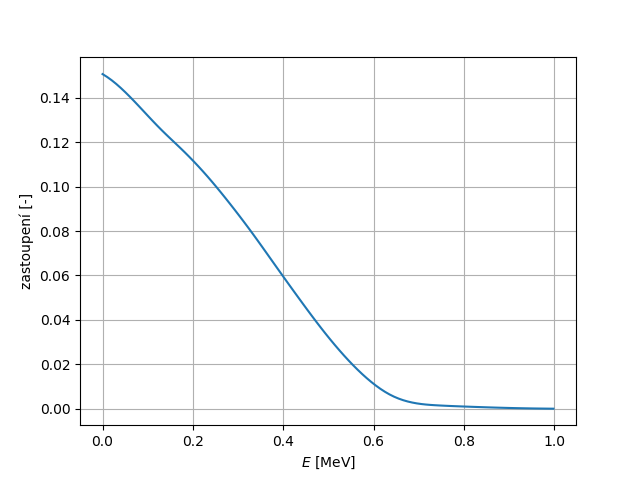
\includegraphics[width=.99\textwidth]{betaSpektrum_Pb.png}
		\caption{}
	\end{subfigure}
	\begin{subfigure}{0.49\textwidth}
		\centering
		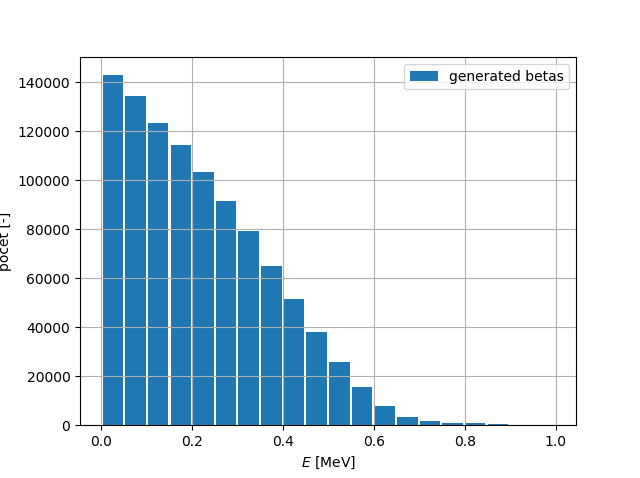
\includegraphics[width=.99\textwidth]{betaNahodnaCisla_Pb.png}
		\caption{}
	\end{subfigure}
\caption{V (a) je originální beta spektrum \ce{^{214}Pb} přebrané z \cite{betaSpektrum}. V (b) je histogram $10^6$ realizací náhodné veličiny řídící se rozdělením, jehož hustota pravděpodobnosti je rovna normovanému beta spektru z (a).}
\label{fig:betaSpektrum_214Pb}
\end{figure}
\begin{figure}[H]
	\centering
	\begin{subfigure}{0.49\textwidth}
		\centering
		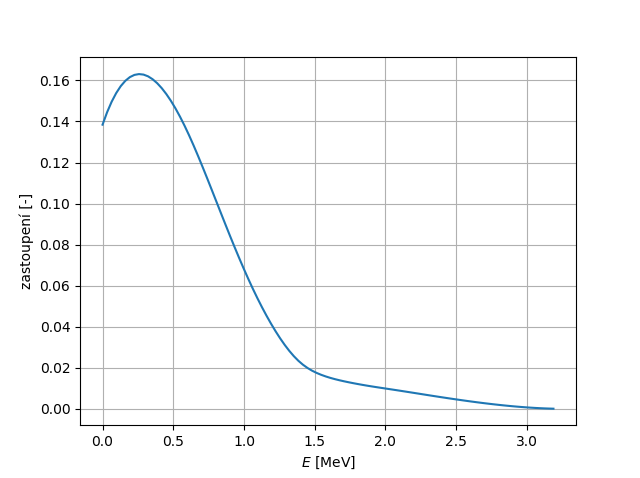
\includegraphics[width=.99\textwidth]{betaSpektrum_Bi.png}
		\caption{}
	\end{subfigure}
	\begin{subfigure}{0.49\textwidth}
		\centering
		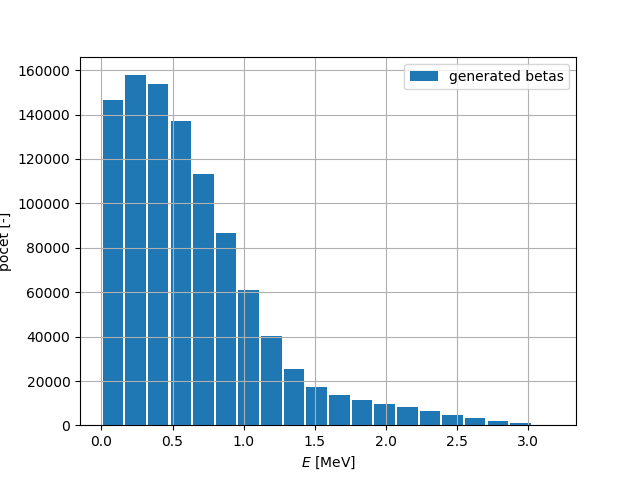
\includegraphics[width=.99\textwidth]{betaNahodnaCisla_Bi.png}
		\caption{}
	\end{subfigure}
	\caption{V (a) je originální beta spektrum \ce{^{214}Bi} přebrané z \cite{betaSpektrum}. V (b) je histogram $10^6$ realizací náhodné veličiny řídící se beta spektrem z (a).}
	\label{fig:betaSpektrum_214Bi}
\end{figure}
\begin{table}[ht]
	\centering
	\caption{Střední energie $\beta$ spekter \ce{^{214}Pb} a \ce{^{214}Bi} vygenerované pomocí metody přijetí-zamítnutí. Maximální chyba určení střední energie je dle Čebyševovy nerovnosti rovna výrazu $\frac{\sigma}{\sqrt{N\cdot \varepsilon}}$, kde $\sigma$ je výběrová směrodatná odchylka, $N=10^6$ je počet vygenerovaných náhodných čísel a $\varepsilon=\num{0,01}$ je hladina významnosti. V posledním sloupci je maximální dosah elektronů s energií $E_{mean}$ přebraný z~\cite{estar}.}
	\label{tab:stredniEnergie}
	\begin{tabular}{lrrr}
		\toprule
		RN&$E_{mean}$ [\si{MeV}]&max. chyba [\si{MeV}]& $R_{max}$ [\si{cm}]\\
		\midrule
		\ce{^{214}Pb}&0,220&0,002&49\\
		\ce{^{214}Bi}&0,639&0,005&231\\
		\bottomrule
	\end{tabular}
\end{table}
\subsubsection{Energetický příspěvek}
%Při určení horní hranice příspěvku $\beta$ záření k dávce byly použity tedy tyto střední energie jejich příslušných spekter (propagace nejistot nebyla uvažována vzhledem k dosti aproximativnímu charakteru výpočtu) a algoritmus uvedený v \ref{navesti:algoritmus_nabiteCastice}. 

Pokud použijeme model výpočtu z kapitoly~\ref{navesti:algoritmus_nabiteCastice}, pak dostaneme výsledky, které lze považovat za maximální odhad deponované energie, protože tento model neuvažuje rozptylování částic do jiných směrů letu než je původní směr letu nabité částice. V algoritmu nahradíme brzdné schopností alfa částic brzdnými schopnostmi elektronů se středními energiemi $\beta$ spekter \cite{estar} a dále je potřeba zavést korekci na fakt, že dosah těchto elektronů (viz tab.~\ref{tab:stredniEnergie}) je větší než rozměry sudu. To znamená, že původní algoritmus by generoval elektrony v místech mimo sud, což je nesmysl. Korekci lze odvodit následující úvahou: uvažujme sférickou slupku s poloměrem $r$ větším než poloměr sudu $R_{sud}$ a menším než polovina výšky sudu $h_{sud}/2$. Pak 

Celkový energetický příspěvek čipu je roven
\begin{equation}
	E_{\beta}=\left(I_{Pb}+I_{Bi}\right)\cdot F\cdot a_0\,,
\end{equation}
se značením stejného významu jako v~\eqref{eq:energetickyPrispevek_integral}. Máme tedy podobně jako v~\eqref{eq:prispevek_alfa}
\begin{empheq}[box=\mymath]{equation}
	\overline{D}_{\beta}=\frac{1}{m_{cip}}E_{beta}\cdot 1,6\times 10^{-13}\frac{1-\exp(-\lambda T)}{\lambda}\,.\label{eq:prispevek_beta}
\end{empheq}
Čára nad $D_{\beta}$ značí, že se jedná o horní maximální odhad.
\subsection{Příspěvek of $\gamma$}
U $\gamma$ záření postupujeme podobným způsobem jako u $\alpha$ s tím rozdílem, že se zde nepočítá s brzdnými schopnostmi, ale s exponenciálním zeslabováním svazku
\begin{align}
	N(d)=N_0e^{-\left(\frac{\mu}{\rho}\right)\cdot\rho\cdot d}\,,
\end{align}
kde $N_0$ je počet fotonů o dané energii $E$ před vstupem materiálu o hustotě $\rho$, $N(d)$ je počet nerozptýlených fotonů po projití materiálu o tloušťce $d$ a $\left(\frac{\mu}{\rho}\right)$ je hmotnostní součinitel zeslabení $\gamma$ záření v uvažovaném materiálu. 

\paragraph{Důležité:} V dalším postupu předpokládáme, že pokud se kvantum $\gamma$ záření rozptýlí, pak již nemůže přispět k dávce absorbované v čipu, tj. uvažujeme úzký svazek. Tato aproximace je částečně ospravedlněna velikou pronikavostí $\gamma$ záření ve vzduchu.

\begin{figure}[ht]
	\centering
	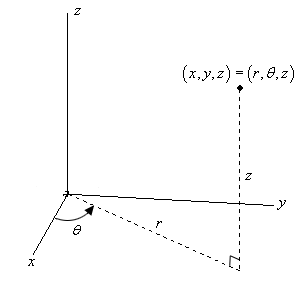
\includegraphics[width=0.4\linewidth]{valcove_souradnice.png}
	\caption{Význam cylindrických souřadnic. \cite{valcovesouradnice}}
	\label{fig:valcovesouradnice}
\end{figure}
Vzhledem k tomu, že sud je rozměrově válec, tak s výhodou využijeme cylindrických souřadnic $(r,\theta, z)$, jejichž význam je znázorněn v obr.~\ref{fig:valcovesouradnice}. 
%V sudu lze očekávat homogenně rozloženou koncentraci radonu, a proto dále není potřeba uvažovat souřadnici
Definujme následující funkci:
\begin{align}
	f(r,z)=\frac{1}{2}\cdot\left(1-\sqrt{\frac{r^2+z^2}{r^2+z^2+R_1^2}}\right)\cdot e^{-\mu\sqrt(r^2+z^2)}\,,\label{eq:gama_geometrie}
\end{align}
kde $\mu$ lineární součinitel zeslabení vzduchu. Tato funkce vyjadřuje, jaký zlomek fotonů vznikající v bodě o daných souřadnicích $r$ a $z$ a libovolné souřadnici $\theta\in[0,2\pi)$ dojde bez rozptýlení ke středu čipu (tím se dopouštíme určité nepřesnosti, jelikož správně bychom měli uvažovat pouze dráhu od místa vzniku k povrchu pouzdra a pak počítat zeslabování v pouzdru). Faktor 
\begin{align}
	\frac{1}{2}\cdot\left(1-\sqrt{\frac{r^2+z^2}{r^2+z^2+R_1^2}}\right)
\end{align}
zohledňuje korekci na prostorový úhel a exponenciela $e^{-\mu\sqrt(r^2+z^2)}$ představuje zeslabení svazku. Funkce $f(r,z)$ je nezávislá na souřadnici $\theta$, jelikož předpokládáme homogenní rozložení koncentrace radonu uvnitř sudu.

Uvažujeme několik zdrojů $\gamma$ záření:
\begin{enumerate}
	\item \emph{vzduch v sudu}, ve kterém je radon o dané koncentrace $a$ a část vznikajících dceřinných produktů, jejichž koncentrace je dána vztahem $a\cdot F$.
	\item \emph{Vnitřní povrch sudu}, na který se deponují dceřinné produkty.
	\item \emph{Povrch pouzdra}, na který se též deponují dceřinné produkty.
	
\end{enumerate}
\paragraph{Zanedbání:} Zanedbáváme $\gamma$ záření vznikající uvnitř čipu a pouzdra a dále neuvažujeme zeslabení svazku uvnitř pouzdra. Tímto odhad dávky od $\gamma$ nadhodnocujeme.
\subsubsection{Vzduch v sudu}
Počet $\gamma$ kvant dané energie, které došly k čipu (při zanedbání pouzdra) v daný časový interval $[t,t+\mathrm{dt}]$, lze vypočítat z
\begin{align}
	N_{air}=a_{air}(t)\cdot Y\cdot 2\int_{R_1}^{R_{sud}}\int_{R_1}^{h_{sud}}f(r,z)\mathrm{dz}\mathrm{dr}\,,
\end{align}
kde $Y$ je výtěžek dané energetické linky a
\begin{align}
a_{air}=\begin{cases}
a & \text{pro $\gamma$ od radonu}\,,\\
a\cdot F & \text{pro $\gamma$ od dcer}\,.
\end{cases}
\end{align}
%Při tomto výpočtu zanedbáváme příspěvky od $\gamma$ záření vznikající v souřadnicích $r\in[0,R_1], z\in[0,R_1]$. Výpočtem bylo ověřeno, že toto zanedbání lze provést.
\subsubsection{Vnitřní povrch sudu}
Koncentrace dceřinných produktů na stěně je rovna
\begin{align}
a_{sud}=a\cdot \frac{V_{sud}}{S_{sud}}\cdot (1-F)\,,\label{eq:povrch_sudu}
\end{align}
kde $S_{sud}=\SI{1,866}{m^2}$ je povrch sudu. Hledaný počet $\gamma$ částic dané energetické linky došlých k čipu:
\begin{equation}
N_{sud}=a_{sud}(t) \cdot Y\cdot 2\left(\int_{0}^{R_{sud}}f(r,h_{sud})\mathrm{dr}+\int_{0}^{h_{sud}}f(R_{sud},z)\mathrm{dz}\right)\,.
\end{equation}
\subsubsection{Povrch pouzdra}
Koncentrace dceřinných produktů na pouzdru je
\begin{align}
a_{pouzdro}=\frac{S_{pouzdro}}{S_{pouzdro}+S_{sud}}\cdot a\cdot \frac{V_{sud}}{S_{pouzdro}}\cdot (1-F)\,,
\end{align}
kde $S_{pouzdro}=\SI{8,81}{cm^2}$ je povrch pouzdra (vypočten ze skutečných rozměrů). Faktor $S_{sud}/(S_{sud}+S_{pouzdro})$ by správně měl být i v \eqref{eq:povrch_sudu}, ale tam může být zanedbán díky jeho blízkosti jedničce.

 $N_{pouzdro}$ bylo odhadnuto následovně:
\begin{align}
N_{pouzdro}=\frac{1}{4}\cdot a_{pouzdro}\cdot Y\,.
\end{align}
Tento odhad se snaží nadhodnocovat příspěvek od dcer deponovaných na pouzdře.

\subsubsection{Příspěvek k dávce}
Nejprve je třeba určit počet částic absorbovaných čipu. To se zjistí pomocí hmotnostního součinitele absorpce $\left(\frac{\mu}{\rho}\right)_{en}$ ze vztahu
\begin{align}
N_{i}^{abs}=N_i\left(1-e^{-\left(\frac{\mu}{\rho}\right)_{en}\cdot \rho_{cip}\cdot 2R_1}\right)\,,
\end{align}
kde $i\in\{air, sud, pouzdro\}$.

V tab.~\ref{tab:gamy} jsou uvedeny nejintenzivnější energetické linky radonu a jeho krátkodobě žijících dceřinných produktů. Některé linky s  blízkou energií byly pro zjednodušení sloučeny dohromady. 
\begin{table}[ht]
	\centering
	\caption{Energie $E$, výtěžek $Y$ a hmotnostní součinitel zeslabení $\frac{\mu}{\rho}$, resp. absorpce $\left(\frac{\mu}{\rho}\right)_{en}$ daného $\gamma$ záření od uvedeného radionuklidu (RN). Řádek s hvězdičkou u RN značí, že u daného radionuklidu bylo z důvodu zjednodušení sloučeno několik blízkých energetických linek dohromady a jejich výtěžky byly sečteny.}
	\label{tab:gamy}
	\begin{tabular}{lrrrr}
		\toprule	 
		RN &  $E$ [keV] &  $Y$ [\%] &       $\left(\frac{\mu}{\rho}\right)$ &    $\left(\frac{\mu}{\rho}\right)_{en}$ \\
		\midrule
		222Rn  &   511 &  7.6 &  0.08712 &  0.02971 \\
		214Pb  &   352 &  37.4 &  0.09800 &  0.02968 \\
		214Pb* &   300 &  27.0 &  0.10670 &  0.02932 \\
		214Bi  &   609 &  46.0 &  0.08055 &  0.02951 \\
		214Bi* &  1180 &  21.0 &  0.05687 &  0.02700 \\
		214Bi  &  1764 &  15.0 &  0.04800 &  0.02445 \\
		214Bi  &  2204 &  5.0 &  0.04447 &  0.02300 \\
		\bottomrule
	\end{tabular}
\end{table}

Dávka od linky s energií $E$ příslušející některému dceřinnému produktu je rovna:
\begin{align}
	D_{progenies}(E)=\frac{1}{m_{cip}}\sum_i N_{i}^{abs}\cdot E\cdot 1,6\times 10^{-16}\frac{1-\exp(-\lambda T)}{\lambda}\,,
\end{align}
dávka od linky \SI{511}{keV} od radonu je následující
\begin{align}
D_{Rn}(511)=\frac{1}{m_{cip}}N_{air}^{abs}\cdot 511\cdot 1,6\times 10^{-16}\frac{1-\exp(-\lambda T)}{\lambda}\,.
\end{align}
Faktor $1,6\times 10^{-16}$ slouží k převodu z \si{keV} na Jouly, $\lambda$ je přeměnová konstanta radonu a $T$ je doba expozice v sekundách.

Celkový příspěvek od $\gamma$ záření k dávce je
\begin{empheq}[box=\mymath]{equation}
D_{\gamma}=D_{Rn}(511)+\sum_{E}D_{progenies}(E)
\end{empheq}
\subsection{Výsledky}
Vypočítal jsem $D_{\alpha}, \overline{D}_{\beta}$ a $D_{\gamma}$ pro $T=\SI{1}{den}$ a pro injektovanou koncentraci $a_0=\SI{1}{kBq\cdot m^{-3}}$:
\begin{align}
	D_{\alpha}&=\SI{5.70}{\mu Gy}\,,\\
	D_{\beta}&=\SI{0.66}{\mu Gy}\,,\\
	D_{\gamma}&=\SI{0.21}{\mu Gy}\,,
\end{align}
což celkově číní
\begin{equation}
	D_{celk}=\SI{6.56}{\mu Gy}\,.
\end{equation}
\subsection{Diskuze}
\subsection{Závěr}
\begin{thebibliography}{Mm99}
	\bibitem{astar} National Institute of Standards and Technology: aStar, Stopping-power and Range Tables for Helium Ions. 14. 5. 2019. Dostupné z \url{https://physics.nist.gov/PhysRefData/Star/Text/ASTAR.html}
	\bibitem{srim} Ziegler, J. F.: SRIM - The Stopping and Range of Ions in Matter. 14. 5. 2019. Dostupné z \url{http://srim.org/} 
	\bibitem{valcovesouradnice} Dawkins, P.: Section 1-12 : Cylindrical Coordinates. Citováno 17. 5. 2019. Dostupné z \url{http://tutorial.math.lamar.edu/Classes/CalcIII/CylindricalCoords.aspx}
	\bibitem{betaSpektrum} Modeste Tchakoua Tchouaso: Odpověď na dotaz "How can I determine the energy spectrum of beta decay?" na webu ResearchGate. Citováno 4. 6. 2019. Dostupné z  \url{https://www.researchgate.net/post/How_can_I_determine_the_energy_spectrum_of_beta_decay}
	\bibitem{rejection} Wikipedia, The Free Encyclopedia: Rejection sampling. Citováno 18. 6. 2019. \url{https://en.wikipedia.org/wiki/Rejection_sampling}
	\bibitem{estar} National Institute of Standards and Technology: eStar, Stopping-power and Range Tables for electrons. 18. 6. 2019. Dostupné z \url{https://physics.nist.gov/PhysRefData/Star/Text/ESTAR.html}
\end{thebibliography}
\end{document}